\documentclass[border=2pt]{standalone}
\usepackage{pgfplots}
\usepgfplotslibrary{fillbetween}
\usetikzlibrary{patterns}
\pgfplotsset{compat=1.18}
\definecolor{paper}{HTML}{18191C}
\definecolor{tile}{HTML}{222429}
\definecolor{rule}{HTML}{454952}
\definecolor{ink}{HTML}{E8EAED}
\definecolor{muted}{HTML}{A3A9B1}
\definecolor{accent}{HTML}{8AB4FF}
\definecolor{red}{HTML}{FF8A80}
\definecolor{green}{HTML}{81C995}
\definecolor{orange}{HTML}{FFAB70}
\definecolor{blue}{HTML}{7CB7FF}
\pagecolor{tile}
\color{ink}
\pgfplotsset{every axis/.append style={axis line style={muted}, tick style={muted}, tick label style={ink, font=\tiny},
  label style={ink, font=\tiny}, title style={ink, font=\tiny}, legend style={fill=tile, draw=rule, text=ink, font=\tiny}},
  every colorbar/.append style={tick label style={font=\tiny}}}
\begin{document}

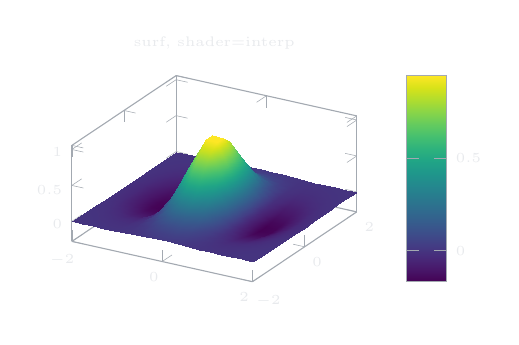
\begin{tikzpicture}
\begin{axis}[width=5.2cm, height=4.2cm, title={surf, shader=interp}, colorbar, colormap/viridis, view={30}{40}]
\addplot3[surf, shader=interp, samples=18, domain=-2:2] {exp(-x^2-y^2)*cos(deg(2*x))};
\end{axis}
\end{tikzpicture}
\end{document}
